\documentclass{article}
\usepackage{epsfig, latexsym}
\usepackage[left=25mm, right=25mm, top=25mm]{geometry}

\begin{document}

\newcommand{\bs}{\backslash}


\title{
\normalsize{EENG 284 -- Spring 2024}\\
\normalsize{Exam 2} \\

\vspace{0.2 in}

Name: \fbox{\rule{2in}{0pt}\rule[-0.5ex]{0pt}{4ex}}
CWID: \fbox{\rule{1in}{0pt}\rule[-0.5ex]{0pt}{4ex}} \\
\date{}
\vspace{0.2 in}
Clearly circle your answer to each question.
}

\maketitle{}

\begin{enumerate}
\item {\bf (3 pts.)} Assuming a word size of 5 bits, interpret 10110 
as a 2's complement number.

\begin{tabular}{p{0.6in} p{0.6in} p{0.6in} p{0.6in} l}
a) -9 & b) -10 & c) -5 & d) 22 & e) None of the above.
\end{tabular}

\item {\bf (3 pts.)} Assuming a word size of 5 bits, determine the 2's complement
representation of -9.

\begin{tabular}{p{0.6in} p{0.6in} p{0.6in} p{0.6in} l}
a) 11011 & b) 10111 & c) 10110 & d) 11001 & e) None of the above.
\end{tabular}

\item {\bf (3 pts.)} How many inputs do the AND gates in a 5:32 decoder have?

\begin{tabular}{p{0.6in} p{0.6in} p{0.6in} p{0.6in} l}
a) 5 & b) 6 & c) 31 & d) 32 & e) None of the above.
\end{tabular}

\item {\bf (3 pts.)} How many 2:1 muxes does it take to build a 32:1 mux?

\begin{tabular}{p{0.6in} p{0.6in} p{0.6in} p{0.6in} l}
a) 3 & b) 7 & c) 15 & d) 31 & e) None of the above.
\end{tabular}

\item {\bf (5 pts.)} Which line of pseudo-code is equivalent to 
the following piece of hardware.  

\includegraphics{./Fig2/conditional2}

\begin{description}
\item{a) } \verb^if (6 < Y) then Z = X+3 else Z = Y+5;^
\item{b) } \verb^if (6 < Y) then Z = Y+5 else Z = Y+3;^
\item{c) } \verb^if (Y < 6) then Z = X+3 else Z = Y+5;^
\item{d) } \verb^if (Y < 6) then Z = Y+5 else Z = Y+3;^
\end{description}

\pagebreak
You are given the following 16:1 multiplexer built from 4:1 multiplexers.
Unfortunately, the select lines were connected in a
most unusual fashion.  Its your job to label each input with the
index which selects it.  Most of the inputs have been omitted
for clarity.

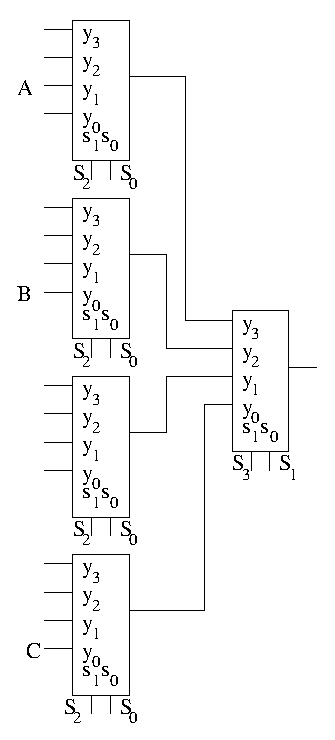
\includegraphics{./Fig2/OddMux}

\item {\bf (3 pts.)} What is the value of the input labeled A?

\begin{tabular}{p{0.6in} p{0.6in} p{0.6in} p{0.6in} l}
a) $y_{7}$ & b) $y_{11}$ & c) $y_{13}$ & d) $y_{14}$ & e) None of the above
\end{tabular}

\item {\bf (3 pts.)} What is the value of the input labeled B?

\begin{tabular}{p{0.6in} p{0.6in} p{0.6in} p{0.6in} l}
a) $y_{1}$ & b) $y_{2}$ & c) $y_{4}$ & d) $y_{8}$ & e) None of the above
\end{tabular}

\item {\bf (3 pts.)} What is the value of the input labeled C?

\begin{tabular}{p{0.6in} p{0.6in} p{0.6in} p{0.6in} l}
a) $y_{0}$ & b) $y_{10}$ & c) $y_{11}$ & d) $y_{12}$ & e) None of the above
\end{tabular}

\pagebreak
For the following problems use the circuit  and timing diagram.
The "c" input of the register's is the control input.  Note one
of the control inputs is G' i(the negation of G) while the other 
is G.

\includegraphics[width=15cm]{./Fig2/seqTiming02.png}


\item {\bf (4 pts.)}What is the value of $P$ at time 15?

\begin{tabular}{p{0.6in} p{0.6in} p{0.6in} p{0.6in} l}
a) 0 & b) 2 & c) 4 & d) 6 & e) none of the above
\end{tabular}

\item {\bf (4 pts.)}What is the value of $Q$ at time 25?

\begin{tabular}{p{0.6in} p{0.6in} p{0.6in} p{0.6in} l}
a) 0 & b) 3 & c) 6 & d) 9 & e) none of the above
\end{tabular}

\item {\bf (4 pts.)}What is the value of $G$ at time 35?

\begin{tabular}{p{0.6in} p{0.6in} p{0.6in} p{0.6in} l}
a) 0 & b) 1 & c) none of the above
\end{tabular}

\item {\bf (4 pts.)}What is the value of $P$ at time 45?

\begin{tabular}{p{0.6in} p{0.6in} p{0.6in} p{0.6in} l}
a) 0 & b) 2 & c) 4 & d) 6 & e) none of the above
\end{tabular}


\pagebreak
You have a digital design which calls for a circuit which performs the 
following task (written as a C if/then statement).

\begin{verbatim}
if      (sum < 6)  z = sum-18
else if (sum < 12) z = sum-12
else if (sum < 18) z = sum-6
else               z = sum
\end{verbatim}

To do this, you have decided on the following architecture.

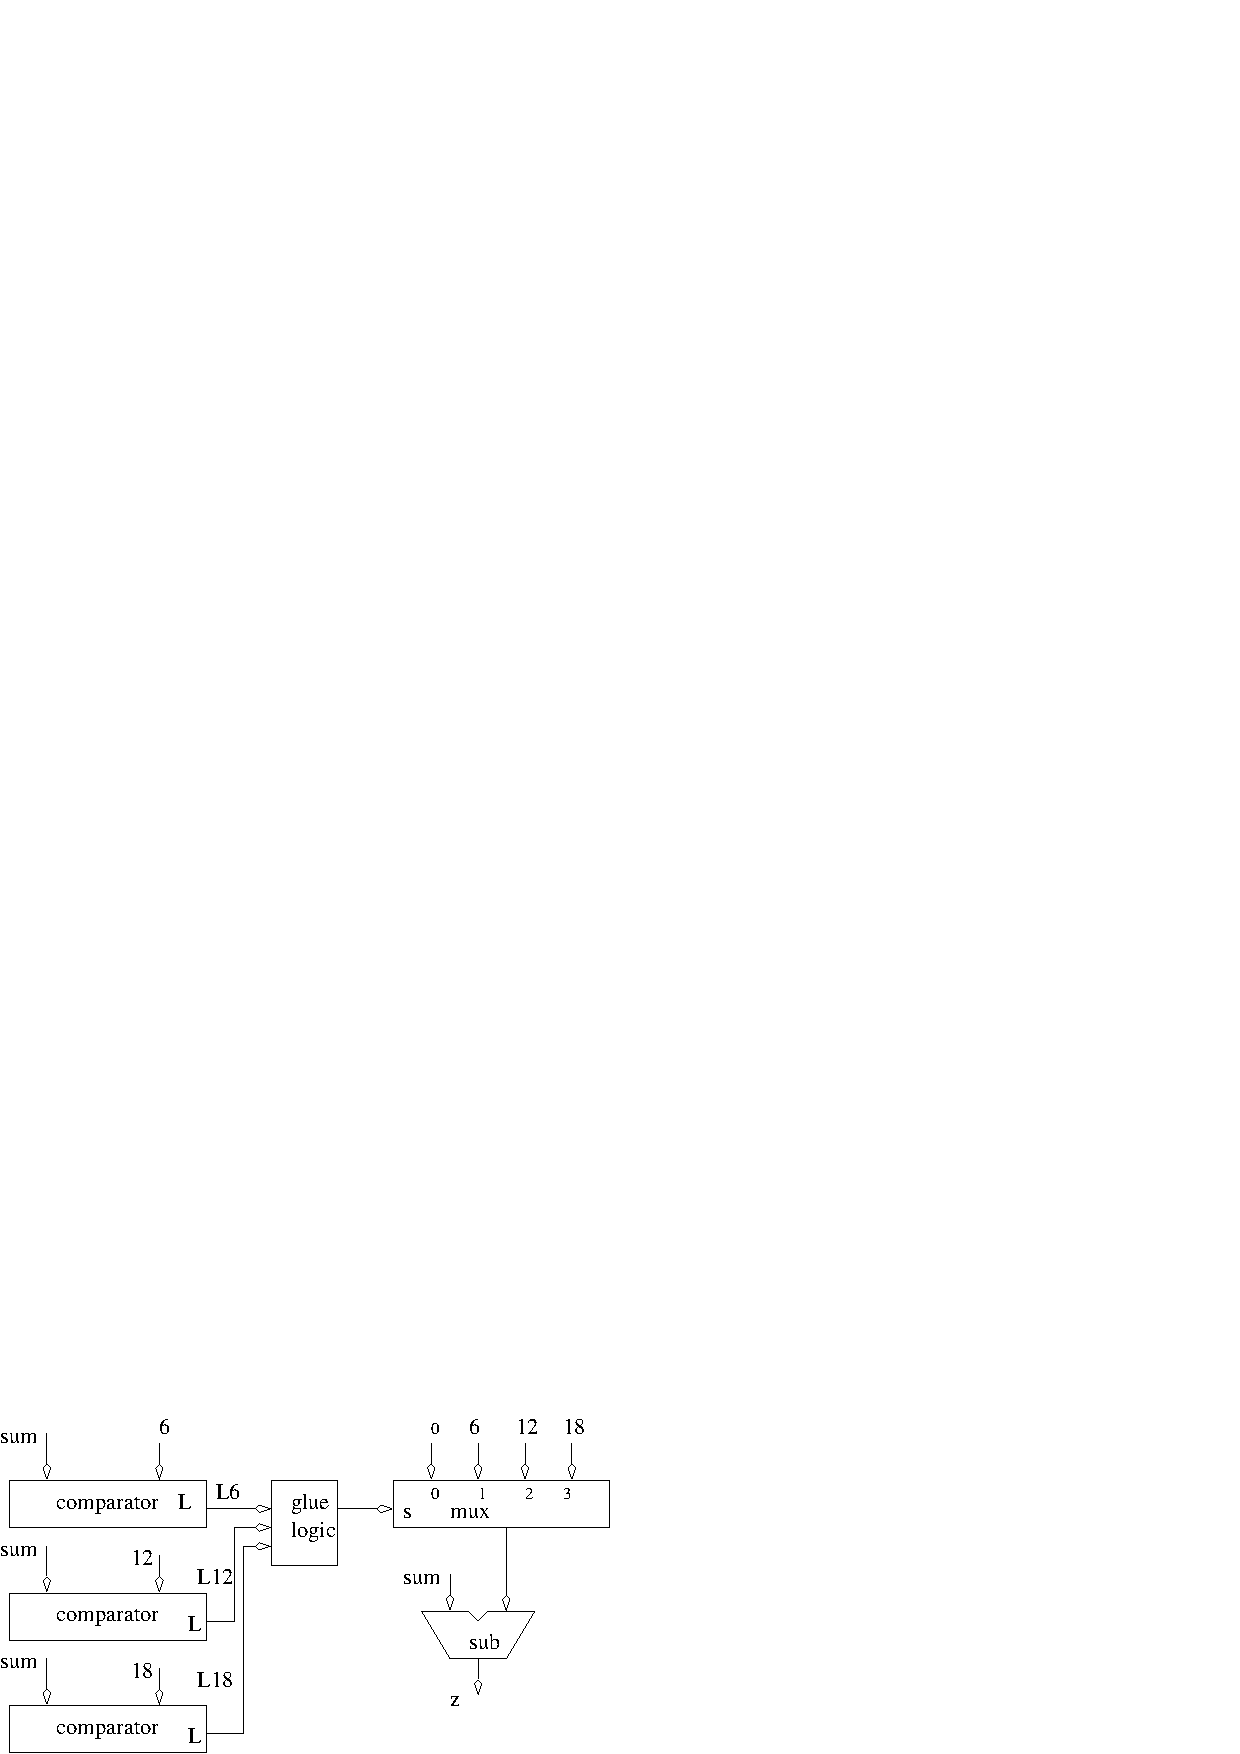
\includegraphics[width=10cm]{./Fig2/if6.png}

It's your job to design to complete the truth table for the 
the \verb+ glue logic+ box.  Show you can do this by completing 
the following three rows.

%\vspace{0.25in}

\begin{tabular}{l|l|l||l}
L6 & L12 & L18 & select \\ \hline
1  & 1   & 1   &   a   \\ \hline
0  & 1   & 1   &   b   \\ \hline
1  & 0   & 1   &   c   \\ 
\end{tabular}

\vspace{0.25in}

\item {\bf (3 pts.)}What is the (decimal) value of a in the truth table?

\begin{tabular}{p{0.6in} p{0.6in} p{0.6in} p{0.6in} l}
a) 0 & b) 1 & c) 2 & d) 3 & e) x  
\end{tabular}

\item {\bf (3 pts.)}What is the (decimal) value of b in the truth table?

\begin{tabular}{p{0.6in} p{0.6in} p{0.6in} p{0.6in} l}
a) 0 & b) 1 & c) 2 & d) 3 & e) x  
\end{tabular}

\item {\bf (3 pts.)}What is the (decimal) value of c in the truth table?

\begin{tabular}{p{0.6in} p{0.6in} p{0.6in} p{0.6in} l}
a) 0 & b) 1 & c) 2 & d) 3 & e) x  
\end{tabular}

\pagebreak
Assume that initial value of Q is 0 (as shown in the figure),
and that the outputs, after a period of rapid toggling, 
end-up at 0.

\scalebox{0.7}{\includegraphics{./Fig2/ExTim4}}

\item {\bf (3 pts.)} What is the value of Q1 at time 25

\begin{tabular}{p{0.75in}p{0.75in}p{0.75in}p{1.25in}}
a) 0 & b) 1 & c) toggling & d) unknown \\
\end{tabular}

\item {\bf (3 pts.)} What is the value of Q1 at time 35

\begin{tabular}{p{0.75in}p{0.75in}p{0.75in}p{1.25in}}
a) 0 & b) 1 & c) toggling & d) unknown \\
\end{tabular}

\item {\bf (3 pts.)} What is the value of Q1 at time 65

\begin{tabular}{p{0.75in}p{0.75in}p{0.75in}p{1.25in}}
a) 0 & b) 1 & c) toggling & d) unknown \\
\end{tabular}

\item {\bf (3 pts.)} What is the value of Q2 at time 25

\begin{tabular}{p{0.75in}p{0.75in}p{0.75in}p{1.25in}}
a) 0 & b) 1 & c) toggling & d) unknown \\
\end{tabular}

\item {\bf (3 pts.)} What is the value of Q2 at time 45

\begin{tabular}{p{0.75in}p{0.75in}p{0.75in}p{1.25in}}
a) 0 & b) 1 & c) toggling & d) unknown \\
\end{tabular}


\pagebreak
For the following problems use the following state table
for the counter.

\begin{tabular}{l|l|l||l|l}
clk             & $C_1 C_0$     & D & $Q^+$  & Note  \\ \hline
0,1,$\downarrow$& xx            & x & Q      & No clk edge  \\ \hline
$\uparrow$      & 00            & x & Q      & Hold  \\  \hline
$\uparrow$      & 01            & x & Q+1    & Count up mod $2^N$	\\  \hline
$\uparrow$      & 10            & x & Q-1    & Count down mod $2^N$	\\  \hline
$\uparrow$      & 11            & D & D      & Parallel load \\
\end{tabular}

\item {\bf (3 pts.)}What is the logic inside \verb+ box + in order
to make the count sequence on Q go from 3 to 10 (inclusive of both)
over and over.

%% \includegraphics[-60mm,23mm][0mm,30.1mm]{./Fig2/OddCnt}
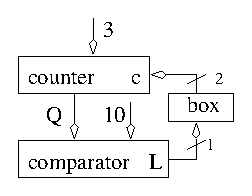
\includegraphics{./Fig2/OddCnt}

\begin{description}
\item{a) }$c_1 = L' \hspace{0.2in} c_0=0$ 
\item{b) }$c_1 = L' \hspace{0.2in} c_0=1$ 
\item{c) }$c_1 = L  \hspace{0.2in} c_0=0$ 
\item{d) }$c_1 = L  \hspace{0.2in} c_0=1$ 
\item{e) }None of the above
\end{description}

Use the timing diagram below as the input to a 4-bit counter with the 
state table given above.  Determine the output sequence Q to answer 
the questions below.

\includegraphics[width=10cm]{./Fig2/CntTime.png}

\item {\bf (3 pt.)}What is the value of $Q$ at time 15?

\begin{tabular}{p{0.6in} p{0.6in} p{0.6in} p{0.6in} l}
a) 0000 & b) 0001 & c) 1110 & d) 1111 & e) None of the above
\end{tabular}

\item {\bf (3 pt.)}What is the value of $Q$ at time 65?

\begin{tabular}{p{0.6in} p{0.6in} p{0.6in} p{0.6in} l}
a) 0000 & b) 0001 & c) 1110 & d) 1111 & e) None of the above
\end{tabular}

\item {\bf (3 pt.)}What is the value of $Q$ at time 85?

\begin{tabular}{p{0.6in} p{0.6in} p{0.6in} p{0.6in} l}
a) 0000 & b) 0001 & c) 1110 & d) 1111 & e) None of the above
\end{tabular}


\end{enumerate}
\end{document}
